SWOT-analysen er en oppsummering av de interne og eksterne analysene. Formålet med analysen er å identifisere hvilke muligheter som ligger til grunn for fremtidig vekst, og trusler ROCKWOOL må ta hensyn til for å kunne nå sitt hovedmål om å bli ledende leverandør av isolasjon.

\begin{figure}[H]
\centering
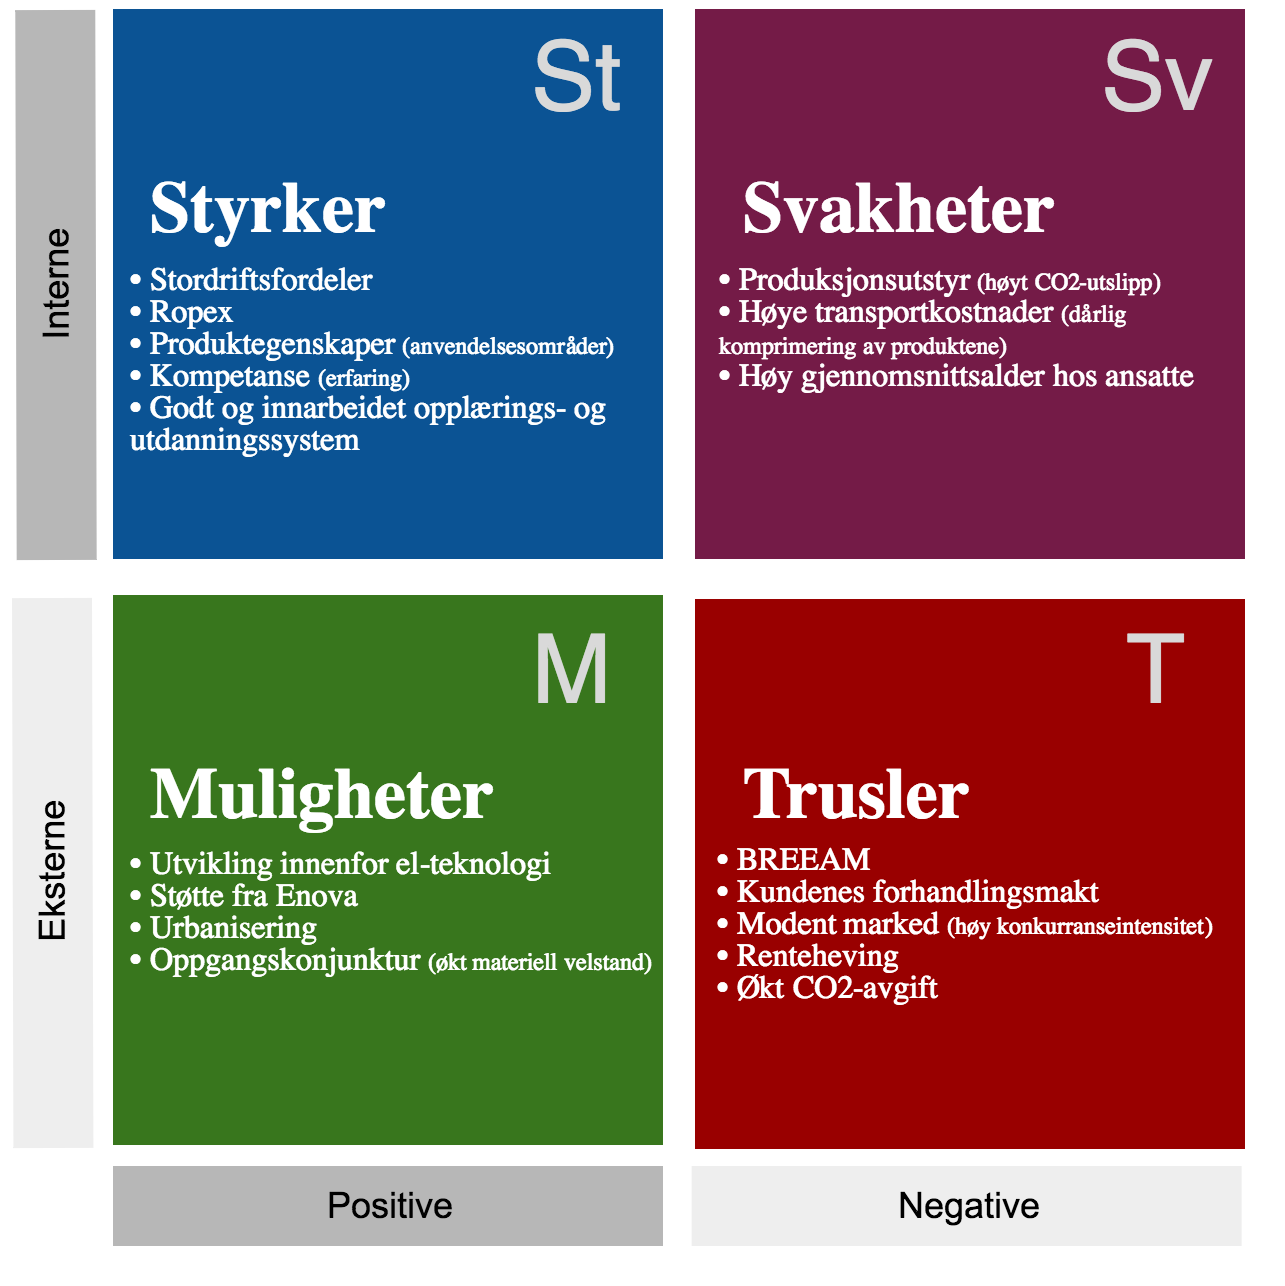
\includegraphics [scale=0.25]{bilder/swot.png}
\caption{SWOT - ROCKWOOL}
\label{fig:swot}
\end{figure}

\indent \newline
De interne analysene viser flere sterke sider ved ROCKWOOL. Ved å være den nest største aktøren i markedet oppnår bedriften stordriftsfordeler som gir lavere enhetskostnader. Dette er en kritisk faktor for å kunne være konkurransedyktig i isolasjonsmarkedet. Gjennom Ropex fokuseres det kontinuerlig på effektivisering av verdikjeden. Bedriften sliter imidlertid med høye transportkostnader grunnet komprimeringsegenskapene til produktet. Produktegenskapene i seg selv gir konkurransefortrinn, men på grunn av for høyt CO2-utslipp i produksjonsprosessen klarer ikke bedriften å utnytte konkurransefortrinnet fullt ut. Kompetansen anses som meget god i form av erfaring og lav turnover. Bedriften bør imidlertid være oppmerksom på den høye gjennomsnittsalderen blant ansatte, og se på muligheter for å bevare kompetansen i årene som kommer.

\indent \newline
Et viktig område identifisert i den eksterne analysen er kundenes forhandlingsmakt og samfunnets fokus på et grønnere miljø. Gjennom økt bruk av BREEAM-sertifisering, stiller entreprenørene høye krav til produktene i form av lavt CO2-utslipp. Disse kravene klarer ikke ROCKWOOL å imøtekomme med nåværende produksjonsteknologi. Markedet opplever lav vekst, og fokus på organisk vekst alene kan skape utfordringer med tanke på å utvide markedsandeler. Videre har jeg identifisert tilgjengelig teknologi innenfor el-smelteovner og utviklingen i transportbransjen som muligheter i dagens markedssituasjon. Ved fremtidige investeringer kan Enova være en potensiell støttespiller.